\documentclass{beamer}
\mode<presentation>
{
	\usetheme{default}
	\usecolortheme{crane}
	\usefonttheme{default}
	\setbeamertemplate{navigation symbols}{}
	\setbeamertemplate{caption}[numbered]
}
\useoutertheme{split}
\setbeamertemplate{navigation symbols}{}
\setbeamertemplate{itemize items}[cirle]
\setbeamertemplate{footline}[frame number]

\usepackage{hyperref}
\usepackage{url}
\usepackage[english]{babel}
\usepackage[utf8x]{inputenc}
\usepackage{caption}
\usepackage{graphicx}
\usepackage[normalem]{ulem}
\usepackage{makecell}

\title[]{IKR}
\author{Jakub Semrič \\ Leo Navel \\ Peter Jareš}
\institute{Brno University of Technology \\ Faculty of Information Technology}
\date{30.\,4.\,2018}

\begin{document}

\begin{frame}
\titlepage
\end{frame}

\begin{frame}{Images Classification}
    \begin{itemize}
        \item SGD (Stochastic Gradient Search)
        \begin{itemize}
            \item linear classifier with SGD
            \item iterative method for minimizing an objective
            \item loss functions\,--\,log, huber, hinge
        \end{itemize}
        \item Random Forest Ensemble
        \item cross validation
        \item data augmentation
    \end{itemize}
\end{frame}

\begin{frame}{Cross Validation}


%\includegraphics{forestCV.png}
\begin{figure}[H]
\centering
\begin{minipage}[b]{0.47\textwidth}
\scalebox{0.37}{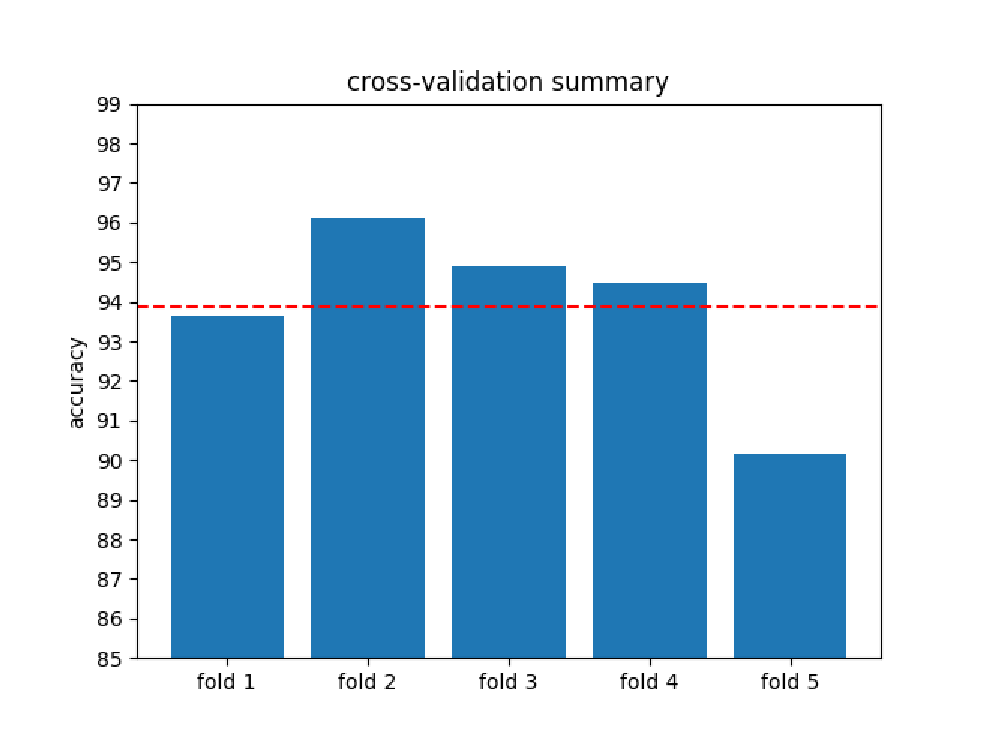
\includegraphics{sgdCV.eps}}
\end{minipage}
\hfill
\begin{minipage}[b]{0.47\textwidth}
\scalebox{0.37}{\includegraphics{forestCV.eps}}
\end{minipage}
\caption{SGD classifier on the left, and Random Forest on the right. The red
dashed line is the mean accuracy of all models.}
\end{figure}
\end{frame}

\begin{frame}{Audio Classification}
    \begin{itemize}
        \item LDA, GMM
    \end{itemize}
\end{frame}

\begin{frame}{Other Approaches}
    \begin{itemize}
        \item deep learning
        \item image preprocessing (SIFT)
        \item massive data augmentation
        \item grid search
    \end{itemize}
\end{frame}

\end{document}
